\chapter {Алгоритми за графи}

\subsection{Алгоритъм на Дейкстра}\index{Дейкстра!алгоритъм}

В този алгоритъм, разглеждаме ориентирани графи $G = (V,E,c)$ с {\em положителни} тегла по ребрата, т.е. $c:E\to\R^+$. 
Целта на алгоритъма е да намерим функции $\delta: V\to\R\cup\{\infty\}$ и $\pi:V\to V\cup\{NULL\}$.
$\delta(v)$ ще дава минималната цена на път от $s$ до $v$. Ако няма път от $s$ до $v$, то $\delta(v)$
ще приема стойност $\infty$. $\pi(v)$ ще дава предшественика на $v$ по път с минимална цена от $s$ до $v$.

\begin{algorithm}
\caption{Алгоритъм на Дейкстра}
\label{alg:dijkstra}

\begin{algorithmic}[1]
  \STATE INIT-SINGLE-SOURCE(G,s)
  
  \WHILE{$V^\prime\neq\emptyset$ \AND $(\exists u\in V^\prime)[\delta(u)<\infty]$}
  \STATE Избираме $u_0\in V^\prime$, за който $ \delta(u_0) = min\{\delta(v)\mid v\in V^\prime\} $
  \STATE $V^\prime := V^\prime\setminus\{u_0\}$
  \FORALL{ $v\in V^\prime $ }
  \IF{$(u_0,v)\in E$ \AND $\delta(v) > \delta(u_0) + c(u_0,v)$}
  \STATE $\delta(v):= \delta(u_0)+c(u_0,v)$
  \STATE $\pi(v) := u_0$
  \ENDIF
  \ENDFOR
  \ENDWHILE
  \RETURN $\delta$
\end{algorithmic}
\end{algorithm}

Във $V^\prime$ може да има останали върхове $v$, но те имат $\delta(v) = \infty$, т.е.
те са недостижими от $s$ и следователно пътят от $s$ до $v$ има дължина $\infty$.

Фигура \ref{fig:dijkstra-table} илюстрира как се променя функцията $\delta$ по време на изпълнението на алгоритъма.
Освен това, с лека модификация на горния алгоритъм, можем да намерим не само стойността на най-късите пътища, но
и списък с ребрата, които участват във всеки оттях. Фигура \ref{fig:dijkstra-graph} илюстрира това.
Ребрата, оцветени в зелено, са тези, които участват в най-късите пътища.

\tikzstyle{weight} = [font=\small]
\tikzstyle{value} = [font=\small]
\tikzstyle{edge} = [draw,thick,-]
\tikzstyle{nodedecorate}=[shape=circle,draw,thick,font=\small]
\tikzstyle{arrowdecorate}=[->,>=stealth,thick]

% Rename: selected --> current
\tikzstyle{selected vertex}=[vertex, fill=yellow!50]
\tikzstyle{selected edge} = [draw,line width=5pt,-,yellow!50]

\tikzstyle{vertex}=[circle,minimum size=15pt,inner sep=0pt]
\tikzstyle{sure vertex} = [vertex, fill=green!30]

\tikzstyle{path edge} = [draw,line width=5pt,-,red!50]

\tikzstyle{sure edge} = [draw,line width=5pt,-,green!30]
% \tikzstyle{ignored edge} = [draw,line width=5pt,-,black!20]


\begin{figure}[!htbp]
  \subfigure{
    \begin{tikzpicture}[]
      
      \foreach \nodename/\x/\y/\direction/\navigate in { a/1/1/above/north,
        b/0/0/left/west, c/1/-1.5/below/south, d/3/1/above/north, e/3/-1.5/below/south, f/5/0.5/right/east, g/5/2.5/right/east}
      {
        \node (\nodename) at (\x,\y) [nodedecorate] {};
        \node [\direction] at (\nodename.\navigate) {$\nodename$};
      }
      %% edges or lines
      \path
      \foreach \startnode/\endnode/\direction/\weight in {b/a/above/7,
        b/c/below/2, c/a/left/4, a/d/below/4, c/e/below/5, d/c/left/8, e/d/right/3}
      {
        (\startnode) edge[arrowdecorate] node[\direction] {$\weight$} (\endnode)
      }
      
      \foreach \startnode/\endnode/\direction/\angle/\weight in {
        a/g/above/15/10, d/f/above/15/5, d/g/above/-15/2, f/d/below/15/1, g/f/right/15/6, e/f/below/-15/7}
      {
        (\startnode) edge[arrowdecorate,bend left=\angle] node[\direction] {$\weight$} (\endnode)
      };
    \end{tikzpicture}
  }
\quad
  \subtable[Разстояния с начален връх $b$]{
    \begin{tabular}[b]{|c|c|c|c|c|c|c|c|c|}
      \hline
      $\delta(a)$ & $\delta(b)$ & $\delta(c)$ & $\delta(d)$ & $\delta(e)$ & $\delta(f)$ & $\delta(g)$\\
      \hline
      $\infty$ & {\bf \framebox{0}} & $\infty$ & $\infty$ & $\infty$ & $\infty$ & $\infty$ \\
      \hline
      7 & $\colon$ & {\bf \framebox{2}} & $\infty$ & $\infty$ & $\infty$ & $\infty$ \\
      \hline
      {\bf \framebox{6}} & $\colon$ & $\colon$ & $\infty$ & 7 & $\infty$ & $\infty$ \\
      \hline
      $\colon$ & $\colon$ & $\colon$ & 10 & {\bf \framebox{7}} & $\infty$ & 16 \\
      \hline
      $\colon$ & $\colon$ & $\colon$ & {\bf \framebox{10}} & $\colon$ & 14 & {\bf 12} \\
      \hline
      $\colon$ & $\colon$ & $\colon$ & $\colon$ & $\colon$ & 14 & {\bf \framebox{12}} \\
      \hline
      $\colon$ & $\colon$ & $\colon$ & $\colon$ & $\colon$ & {\bf \framebox{14}} & $\colon$ \\
      \hline
      $\colon$ & $\colon$ & $\colon$ & $\colon$ & $\colon$ & $\colon$ & $\colon$ \\
      \hline
    \end{tabular}
  }
  \caption{Алгоритъм на Дейкстра}
  \label{fig:dijkstra-table}
\end{figure}


\begin{figure}[!htbp]
  \index{Дейкстра!алгоритъм}
  

\subfigure[Започваме от съседите на $a$]{
  \begin{tikzpicture}[scale=0.9]
    % nodes
    \foreach \nodename/\x/\y/\value/\direction/\navigate/\color in { 
      a/0/0/0/above/north/green, 
      b/-1/1/\infty/left/west/black, 
      c/2.5/1/\infty/above/north/black, 
      d/2/-0.5/\infty/below/south/black,
      e/-1/-0.5/\infty/below/south/black, 
      f/0.5/2/\infty/above/north/black,
      g/0/-1.8/\infty/below/south/black, 
      h/2.5/-1.8/\infty/right/east/black}
    {
        \node[vertex, nodedecorate, fill=\color!25] (\nodename) at (\x,\y) {$\value$};
        \node [\direction] at (\nodename.\navigate) {$\nodename$};
      };
      % edges
      \path
      \foreach \startnode/\endnode/\direction/\angle/\weight in {
        e/b/left/15/5, e/g/below/-15/3, d/g/below/15/2, 
        g/a/left/15/2, a/g/right/30/9, f/c/below/-15/1,
        c/f/above/-30/5, c/h/right/15/2, c/d/above/-15/1,
        f/d/left/-15/4, a/b/below/0/2, b/f/above/0/1, 
        a/d/above/0/8}
      {
        (\startnode) edge[arrowdecorate,bend left=\angle] node[\direction] {$\weight$} (\endnode)
      };
    \end{tikzpicture}
  }
  \subfigure[$b$ е най-близко до $a$]{
    \begin{tikzpicture}[scale=0.9]
      %nodes
      \foreach \nodename/\x/\y/\value/\direction/\navigate/\color in { 
        a/0/0/0/above/north/green, 
        b/-1/1/2/left/west/yellow, 
        c/2.5/1/\infty/above/north/black, 
        d/2/-0.5/8/below/south/yellow,
        e/-1/-0.5/\infty/below/south/black, 
        f/0.5/2/\infty/above/north/black, 
        g/0/-1.8/9/below/south/yellow, 
        h/2.5/-1.8/\infty/right/east/black}
      {
        \node[vertex, nodedecorate, fill=\color!25] (\nodename) at (\x,\y) {$\value$};
        \node [\direction] at (\nodename.\navigate) {$\nodename$};
      };

      \path
      \foreach \startnode/\endnode/\direction/\angle in {
        a/g/right/30, a/b/above/0, a/d/above/0}
      {
        (\startnode) edge[selected edge,bend left=\angle] node[\direction] {} (\endnode)
      };
      %edges
      \path
      \foreach \startnode/\endnode/\direction/\angle/\weight in {
        e/b/left/15/5, e/g/below/-15/3, d/g/below/15/2, g/a/left/15/2, a/g/right/30/9, f/c/below/-15/1, c/f/above/-30/5,
        c/h/right/15/2, c/d/above/-15/1, f/d/left/-15/4, a/b/below/0/2, b/f/above/0/1,  a/d/above/0/8}
      {
        (\startnode) edge[arrowdecorate,bend left=\angle] node[\direction] {$\weight$} (\endnode)
      };
    \end{tikzpicture}
  }
  \subfigure[Най-къс път до $f$]{
    \begin{tikzpicture}[scale=0.9]
      %nodes
      \foreach \nodename/\x/\y/\value/\direction/\navigate/\color in { 
        a/0/0/0/above/north/green, 
        b/-1/1/2/left/west/green,
        c/2.5/1/\infty/above/north/black, 
        d/2/-0.5/8/below/south/yellow,
        e/-1/-0.5/\infty/below/south/black, 
        f/0.5/2/3/above/north/yellow, 
        g/0/-1.8/9/below/south/yellow, 
        h/2.5/-1.8/\infty/right/east/black}
      {
        \node[vertex, nodedecorate, fill=\color!25] (\nodename) at (\x,\y) {$\value$};
        \node [\direction] at (\nodename.\navigate) {$\nodename$};
      };
      \path
      (a) edge[sure edge] node[] {} (b);
      \path
      \foreach \startnode/\endnode/\direction/\angle in {
        a/g/right/30, a/d/above/0}
      {
        (\startnode) edge[selected edge,bend left=\angle] node[\direction] {} (\endnode)
      };
      \path
      \foreach \startnode/\endnode/\direction/\angle in {
         b/f/above/0}
      {
        (\startnode) edge[selected edge, bend left=\angle] node[\direction] {} (\endnode)
      };
      %edges
      \path
      \foreach \startnode/\endnode/\direction/\angle/\weight in {
        e/b/left/15/5, e/g/below/-15/3, d/g/below/15/2, g/a/left/15/2, a/g/right/30/9, f/c/below/-15/1, c/f/above/-30/5,
        c/h/right/15/2, c/d/above/-15/1, f/d/left/-15/4, a/b/below/0/2, b/f/above/0/1,  a/d/above/0/8}
      {
        (\startnode) edge[arrowdecorate,bend left=\angle] node[\direction] {$\weight$} (\endnode)
      };
    \end{tikzpicture}
  }
  \subfigure[По-къс път до $d$ и $c$]{
    \begin{tikzpicture}[scale=0.9]
      % nodes
      \foreach \nodename/\x/\y/\value/\direction/\navigate/\color in { 
        a/0/0/0/above/north/green,
        b/-1/1/2/left/west/green,
        c/2.5/1/4/above/north/yellow, 
        d/2/-0.5/7/below/south/yellow,
        e/-1/-0.5/\infty/below/south/black, 
        f/0.5/2/3/above/north/green, 
        g/0/-1.8/9/below/south/yellow, 
        h/2.5/-1.8/\infty/right/east/black}
      {
        \node[vertex, nodedecorate, fill=\color!25] (\nodename) at (\x,\y) {$\value$};
        \node [\direction] at (\nodename.\navigate) {$\nodename$};
      };
      \path
      (a) edge[sure edge] node[] {} (b)
      (b) edge[sure edge] node[] {} (f);
      
      \path
      \foreach \startnode/\endnode/\direction/\angle in {
        a/d/above/0}
      {
        (\startnode) edge[path edge,bend left=\angle] node[\direction] {} (\endnode)
      };
      \path
      \foreach \startnode/\endnode/\direction/\angle in {f/c/below/-15/1, f/d/left/-15/4, a/g/right/30}
      {
        (\startnode) edge[selected edge, bend left=\angle] node[\direction] {} (\endnode)
      };
      %edges
      \path
      \foreach \startnode/\endnode/\direction/\angle/\weight in {
        e/b/left/15/5, e/g/below/-15/3, d/g/below/15/2, g/a/left/15/2, a/g/right/30/9, f/c/below/-15/1, c/f/above/-30/5,
        c/h/right/15/2, c/d/above/-15/1, f/d/left/-15/4, a/b/below/0/2, b/f/above/0/1,  a/d/above/0/8}
      {
        (\startnode) edge[arrowdecorate,bend left=\angle] node[\direction] {$\weight$} (\endnode)
      };
    \end{tikzpicture}
  }
  \subfigure[По-къс път до $d$ и $h$]{
    \begin{tikzpicture}[scale=0.9]
      % nodes
      \foreach \nodename/\x/\y/\value/\direction/\navigate/\color in { 
        a/0/0/0/above/north/green,
        b/-1/1/2/left/west/green,
        c/2.5/1/4/above/north/green,
        d/2/-0.5/5/below/south/yellow,
        e/-1/-0.5/\infty/below/south/black, 
        f/0.5/2/3/above/north/green, 
        g/0/-1.8/9/below/south/yellow, 
        h/2.5/-1.8/6/right/east/yellow}
      {
        \node[vertex, nodedecorate, fill=\color!25] (\nodename) at (\x,\y) {$\value$};
        \node [\direction] at (\nodename.\navigate) {$\nodename$};
      };
      \path
      (a) edge[sure edge] node[] {} (b)
      (b) edge[sure edge] node[] {} (f)
      (f) edge[sure edge, bend left=-15] node[] {} (c);
      
      \path
      \foreach \startnode/\endnode/\direction/\angle in {f/d/left/-15/4, a/d/above/0
        }
      {
        (\startnode) edge[path edge,bend left=\angle] node[\direction] {} (\endnode)
      };
      \path
      \foreach \startnode/\endnode/\direction/\angle in {c/d/above/-15/1,  c/f/above/-30/5, c/h/right/15/2, a/g/right/30}
      {
        (\startnode) edge[selected edge, bend left=\angle] node[\direction] {} (\endnode)
      };
      %edges
      \path
      \foreach \startnode/\endnode/\direction/\angle/\weight in {
        e/b/left/15/5, e/g/below/-15/3, d/g/below/15/2, g/a/left/15/2, a/g/right/30/9, f/c/below/-15/1, c/f/above/-30/5,
        c/h/right/15/2, c/d/above/-15/1, f/d/left/-15/4, a/b/below/0/2, b/f/above/0/1,  a/d/above/0/8}
      {
        (\startnode) edge[arrowdecorate,bend left=\angle] node[\direction] {$\weight$} (\endnode)
      };
    \end{tikzpicture}
  }
  \subfigure[По-къс път до $g$]{
    \begin{tikzpicture}[scale=0.9]
      %nodes
      \foreach \nodename/\x/\y/\value/\direction/\navigate/\color in { 
        a/0/0/0/above/north/green, 
        b/-1/1/2/left/west/green,
        c/2.5/1/4/above/north/green,
        d/2/-0.5/5/below/south/green,
        e/-1/-0.5/\infty/below/south/black, 
        f/0.5/2/3/above/north/green, 
        g/0/-1.8/7/below/south/yellow,
        h/2.5/-1.8/6/right/east/yellow}
      {
        \node[vertex, nodedecorate, fill=\color!25] (\nodename) at (\x,\y) {$\value$};
        \node [\direction] at (\nodename.\navigate) {$\nodename$};
      };
      \path
      (a) edge[sure edge] node[] {} (b)
      (b) edge[sure edge] node[] {} (f)
      (f) edge[sure edge, bend left=-15] node[] {} (c)
      (c) edge[sure edge, bend left=-15] node[] {} (d);
      
      \path
      \foreach \startnode/\endnode/\direction/\angle in {f/d/left/-15, a/g/right/30, a/d/above/0, c/f/above/-30
        }
      {
        (\startnode) edge[path edge,bend left=\angle] node[] {} (\endnode)
      };
      \path
      \foreach \startnode/\endnode/\direction/\angle in {d/g/below/15/2, c/h/right/15}
      {
        (\startnode) edge[selected edge, bend left=\angle] node[\direction] {} (\endnode)
      };
      %edges
      \path
      \foreach \startnode/\endnode/\direction/\angle/\weight in {
        e/b/left/15/5, e/g/below/-15/3, d/g/below/15/2, g/a/left/15/2, a/g/right/30/9, f/c/below/-15/1, c/f/above/-30/5,
        c/h/right/15/2, c/d/above/-15/1, f/d/left/-15/4, a/b/below/0/2, b/f/above/0/1,  a/d/above/0/8}
      {
        (\startnode) edge[arrowdecorate,bend left=\angle] node[\direction] {$\weight$} (\endnode)
      };
    \end{tikzpicture}
  }
  \subfigure[$h$ е задънена улица]{
    \begin{tikzpicture}[scale=0.9]
      %nodes
      \foreach \nodename/\x/\y/\value/\direction/\navigate/\color in { 
        a/0/0/0/above/north/green, 
        b/-1/1/2/left/west/green,
        c/2.5/1/4/above/north/green, 
        d/2/-0.5/5/below/south/green,
        e/-1/-0.5/\infty/below/south/black, 
        f/0.5/2/3/above/north/green, 
        g/0/-1.8/7/below/south/yellow,
        h/2.5/-1.8/6/right/east/green}
      {
        \node[vertex, nodedecorate, fill=\color!25] (\nodename) at (\x,\y) {$\value$};
        \node [\direction] at (\nodename.\navigate) {$\nodename$};
      };
      \path
      (a) edge[sure edge] node[] {} (b)
      (b) edge[sure edge] node[] {} (f)
      (f) edge[sure edge, bend left=-15] node[] {} (c)
      (c) edge[sure edge, bend left=-15] node[] {} (d)
      (c) edge[sure edge, bend left=15] node[] {} (h);
      
      \path
      \foreach \startnode/\endnode/\direction/\angle in {f/d/left/-15, a/g/right/30, a/d/above/0, c/f/above/-30
        }
      {
        (\startnode) edge[path edge,bend left=\angle] node[] {} (\endnode)
      };
      \path
      \foreach \startnode/\endnode/\direction/\angle in {d/g/below/15/2}
      {
        (\startnode) edge[selected edge, bend left=\angle] node[\direction] {} (\endnode)
      };
      %edges
      \path
      \foreach \startnode/\endnode/\direction/\angle/\weight in {
        e/b/left/15/5, e/g/below/-15/3, d/g/below/15/2, g/a/left/15/2, a/g/right/30/9, f/c/below/-15/1, c/f/above/-30/5,
        c/h/right/15/2, c/d/above/-15/1, f/d/left/-15/4, a/b/below/0/2, b/f/above/0/1,  a/d/above/0/8}
      {
        (\startnode) edge[arrowdecorate,bend left=\angle] node[\direction] {$\weight$} (\endnode)
      };
    \end{tikzpicture}
  }
  \subfigure[$e$ не е достижим]{
    \begin{tikzpicture}[scale=0.9]
      %nodes
      \foreach \nodename/\x/\y/\value/\direction/\navigate/\color in { 
        a/0/0/0/above/north/green,
        b/-1/1/2/left/west/green,
        c/2.5/1/4/above/north/green, 
        d/2/-0.5/5/below/south/green,
        e/-1/-0.5/\infty/below/south/black, 
        f/0.5/2/3/above/north/green, 
        g/0/-1.8/7/below/south/green,
        h/2.5/-1.8/6/right/east/green}
      {
        \node[vertex, nodedecorate, fill=\color!25] (\nodename) at (\x,\y) {$\value$};
        \node [\direction] at (\nodename.\navigate) {$\nodename$};
      };
      \path
      (a) edge[sure edge] node[] {} (b)
      (b) edge[sure edge] node[] {} (f)
      (f) edge[sure edge, bend left=-15] node[] {} (c)
      (c) edge[sure edge, bend left=-15] node[] {} (d)
      (c) edge[sure edge, bend left=15] node[] {} (h)
      (d) edge[sure edge, bend left=15] node[] {} (g);
      
      \path
      \foreach \startnode/\endnode/\direction/\angle in {f/d/left/-15, a/g/right/30, a/d/above/0, c/f/above/-30
        }
      {
        (\startnode) edge[path edge,bend left=\angle] node[] {} (\endnode)
      };
      \path
      \foreach \startnode/\endnode/\direction/\angle in {g/a/left/15}
      {
        (\startnode) edge[selected edge, bend left=\angle] node[\direction] {} (\endnode)
      };
      %edges
      \path
      \foreach \startnode/\endnode/\direction/\angle/\weight in {
        e/b/left/15/5, e/g/below/-15/3, d/g/below/15/2, g/a/left/15/2, a/g/right/30/9, f/c/below/-15/1, c/f/above/-30/5,
        c/h/right/15/2, c/d/above/-15/1, f/d/left/-15/4, a/b/below/0/2, b/f/above/0/1,  a/d/above/0/8}
      {
        (\startnode) edge[arrowdecorate,bend left=\angle] node[\direction] {$\weight$} (\endnode)
      };
    \end{tikzpicture}
  }
  \subfigure[Краен резултат]{
    \begin{tikzpicture}[scale=0.9]
      %nodes
      \foreach \nodename/\x/\y/\value/\direction/\navigate/\color in { 
        a/0/0/0/above/north/green, b/-1/1/2/left/west/green,
        c/2.5/1/4/above/north/green, d/2/-0.5/5/below/south/green,
        e/-1/-0.5/\infty/below/south/black, f/0.5/2/3/above/north/green, 
        g/0/-1.8/7/below/south/green, h/2.5/-1.8/6/right/east/green}
      {
        \node[vertex, nodedecorate, fill=\color!25] (\nodename) at (\x,\y) {$\value$};
        \node [\direction] at (\nodename.\navigate) {$\nodename$};
      };
      \path
      (a) edge[sure edge] node[] {} (b)
      (b) edge[sure edge] node[] {} (f)
      (f) edge[sure edge, bend left=-15] node[] {} (c)
      (c) edge[sure edge, bend left=-15] node[] {} (d)
      (c) edge[sure edge, bend left=15] node[] {} (h)
      (d) edge[sure edge, bend left=15] node[] {} (g);
      
      \path
      \foreach \startnode/\endnode/\direction/\angle in {f/d/left/-15, a/g/right/30, a/d/above/0, c/f/above/-30, g/a/above/15
        }
      {
        (\startnode) edge[path edge,bend left=\angle] node[] {} (\endnode)
      };
      \path
      \foreach \startnode/\endnode/\direction/\angle in {}
      {
        (\startnode) edge[selected edge, bend left=\angle] node[\direction] {} (\endnode)
      };
      %edges
      \path
      \foreach \startnode/\endnode/\direction/\angle/\weight in {
        e/b/left/15/5, e/g/below/-15/3, d/g/below/15/2, g/a/left/15/2, a/g/right/30/9, f/c/below/-15/1, c/f/above/-30/5,
        c/h/right/15/2, c/d/above/-15/1, f/d/left/-15/4, a/b/below/0/2, b/f/above/0/1,  a/d/above/0/8}
      {
        (\startnode) edge[arrowdecorate,bend left=\angle] node[\direction] {$\weight$} (\endnode)
      };
    \end{tikzpicture}
  }

%%% Local Variables: 
%%% mode: latex
%%% TeX-master: "discrete-math"
%%% End: 

  \caption{Алгоритъм на Дейкстра запазващ минималните пътища}
  \label{fig:dijkstra-graph}
\end{figure}

\begin{problem}
  Дайте пример за насочен граф с отрицателен цикъл, при който алгоритъмът на Дейкстра не дава правилния резултат.
\end{problem}

\newpage
\subsection{Алгоритъм на Белман-Форд}\index{Белман-Форд!алгоритъм}

Алгоритъмът на Дейкстра работи само за графи с {\em положителни} тегла по ребрата.
Сега ще разгледаме един алгоритъм, който работи и за графи с отрицателни тегла по ребрата.
Отново искаме да намерим минималните разстояния на пътищата с начало върха $s$, но
алгоритъмът отговаря на въпроса дали има отрицателен цикъл в графа. Ако такъв съществува, то няма решение на проблема.
Ако отрицателен цикъл не съществува, то алгоритъмът намира най-късите пътища в графа.


\begin{algorithm}
  \caption{Белман-Форд}
  \label{alg:belman-ford}
  
  \begin{algorithmic}[1]
    
    \STATE INIT-SINGLE-SOURCE(G,s)
    
    \FOR{$i:=1$ to $\abs{V}-1$}
    \FORALL{$(u,v)\in E$}
    \IF{$\delta(v) > \delta(u) + c(u,v)$}
    \STATE $\delta(v) := \delta(u) + c(u,v)$
    \STATE $\pi(v) := u$
    \ENDIF
    \ENDFOR
    \ENDFOR
    
    \COMMENT{Проверка за отрицателен цикъл}
    \FORALL{$(u,v)\in E$}
    \IF {$\delta(v) > \delta(u) + c(u,v)$}
    \RETURN \FALSE
    \ENDIF
    \ENDFOR
    \RETURN \TRUE
    
  \end{algorithmic}
\end{algorithm}

% \begin{enumerate}[1)]
%   \item
%     Дефинираме функция $\delta:V\to\R^+\cup\{\infty\}$ като
%     \[\delta(u)=
%     \begin{cases}
%       0 & \text{, ако } u = s\\
%       \infty & \text{, иначе}
%     \end{cases}
%     \]
%   Тъй като $V$ е крайно множество, можем да представим $\delta$ като масив.
%   \item
%     За всяко ребро $(u,v)\in E$,
%         \[\delta(v) :=
%         \begin{cases}
%           \delta(u) + c(u,v) & \text{, ако } \delta(v) > \delta(u) + c(u,v)\\
%           \delta(v) & \text{, иначе}
%         \end{cases}
%         \]
%   \item
%     Стъпка 2) се изпълнява общо $\nu- 1$ пъти.
%   \item
%     За всяко ребро $(u,v)\in E$, проверяваме дали $\delta(v) > \delta(u) + c(u,v)$.
%     Ако намерим такова ребро, то процедурата връща $FALSE$, иначе връща $TRUE$.
% \end{enumerate}

Твърдим, че в масива $\delta$ ще се съдържат търсените минималните пътища, яко няма отрицателни цикли достижими от $s$ в графа.
Тъй като всеки прост път има дължина не по-голяма от $\nu-1$, то след завършване на процедурата ще имаме минималните 
дължини на пътищата от зададения връх $s$ до всички останали върхове в графа.

Сега да разгледаме случая на граф с отрицателен цикъл достижим от $s$, $c = (v_0,\dots,v_k)$ и $v_0 = v_k$, т.е.
\[\sum^{k}_{i=1}c(v_{i-1},v_i) < 0.\]
Да допуснем, че процедурата връща $TRUE$. Тогава $\delta(v_i) \leq \delta(v_{i-1}) + c(v_{i-1},v_i)$, за всяко $i=1,\dots,k$ и
\[\sum^{k}_{i=1} \delta(v_i) \leq \sum^{k}_{i=1}\delta(v_{i-1}) + \sum^{k}_{i=1}c(v_{i-1},v_i).\]
Тъй като $v_0 = v_k$, $\sum^{k}_{i=1} d(v_i) = \sum^{k}_{i=1}d(v_{i-1})$.
Получаваме, че $0 \leq \sum^{k}_{i=1}c(v_{i-1},v_i)$, което е противоречие с отицателността на цикъла.
Фигура \ref{fig:bellman-ford-negative-cycle} илюстрира този случай.
Както забелязахме при алгоритъма на Дейкстра, и тук можем да намерим не само дължините на най-късите пътища, но
и спъсъка на ребрата, участващи в тях. Фигура \ref{fig:bellman-ford-graph} илюстрира този проблем. 
Останалите накрая оцветени в синьо ребра участват в най-късите пътища.



\begin{figure}[!htbp]
  \subfigure{
  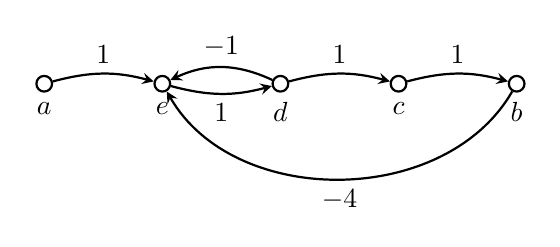
\begin{tikzpicture}
    [nodedecorate/.style={shape=circle,inner sep=2pt,draw,thick},%
    arrowdecorate/.style={->,>=stealth,thick}]
    %% nodes or vertices
    
    \foreach \nodename/\x/\y/\direction/\navigate in { a/0/0/below/south,
      b/6/0/below/south, c/4.5/0/below/south, d/3/0/below/south, e/1.5/0/below/south}
    {
      \node (\nodename) at (\x,\y) [nodedecorate] {};
      \node [\direction] at (\nodename.\navigate) {$\nodename$};
    }
    %% edges or lines
    \path
    \foreach \startnode/\endnode/\direction/\angle/\weight in {
      a/e/above/15/1, d/e/above/-25/-1, e/d/below/-15/1,  d/c/above/15/1, c/b/above/15/1, b/e/below/60/-4}
    {
      (\startnode) edge[arrowdecorate,bend left=\angle] node[\direction] {$\weight$} (\endnode)
    };
    ;
  \end{tikzpicture}
}
\quad
\subfigure{
      \begin{tabular}{|c|c|c|c|c|}
      \hline
      $\delta(a)$ & $\delta(b)$ & $\delta(c)$ & $\delta(c)$ & $\delta(e)$ \\
      \hline
      0 & $\infty$ & $\infty$ & $\infty$ & {\bf \framebox{1}}\\
      \hline
      \hline
      $\colon$ & \framebox{$\infty$} & $\infty$ & $\infty$ & 1\\
      $\colon$ & $\infty$ & \framebox{$\infty$} & $\infty$ & 1\\
      $\colon$ & $\infty$ & $\infty$ & {\bf \framebox{2}} & 1\\
      $\colon$ & $\infty$ & $\infty$ & 2 & \framebox{1}\\
      \hline\hline
      $\colon$ & \framebox{$\infty$} & $\infty$ & 2 & 1\\
      $\colon$ & $\infty$ & {\bf \framebox{3}} & 2 & 1\\
      $\colon$ & $\infty$ & 3 & \framebox{2} & 1\\
      $\colon$ & $\infty$ & $\infty$ & 2 & \framebox{1}\\
      \hline\hline
      $\colon$ & {\bf \framebox{4}} & 3 & 2 & 1\\
      $\colon$ & 4 & \framebox{3} & 2 & 1\\
      $\colon$ & 4 & 3 & \framebox{2} & 1\\
      $\colon$ & 4 & 3 & 2 & {\bf \framebox{0}}\\
      \hline\hline
    \end{tabular}
  }
  \caption{Алгоритъм на Белман-Форд върху ориентиран граф с отрицателен цикъл}
  \label{fig:bellman-ford-negative-cycle}
\end{figure}


\begin{figure}[!htbp]
  
\begin{subfigure}[b]{0.3\textwidth}
    \begin{tikzpicture}[scale=0.9]
      %% nodes or vertices
      
      \foreach \nodename/\value/\x/\y/\direction/\navigate/\color in { 
        s/0/0/0/left/west/green, 
        x/\infty/3.5/1.5/above/north/black,
        y/\infty/1/-1.5/below/south/black,
        t/\infty/1/1.5/above/north/black, 
        z/\infty/3.5/-1.5/below/south/black}
      {
        \node[vertex, nodedecorate, fill=\color!25] (\nodename) at (\x,\y) {$\value$};
        \node [\direction] at (\nodename.\navigate) {$\nodename$};
      }
      % edges or lines
      \path
      \foreach \startnode/\endnode/\direction/\angle/\weight in {
        s/t/left/15/6, s/y/left/-25/7, y/z/below/0/9,  t/y/left/0/8, t/x/above/30/5, x/t/above/30/-2, z/x/right/0/7,
        z/s/below/0/2, y/x/below/-3, t/z/right/15/-4
      }
      {
        (\startnode) edge[arrowdecorate,bend left=\angle] node[\direction] {$\weight$} (\endnode)
      };
      ;
    \end{tikzpicture}
    \caption{Начален връх е $s$}
  \end{subfigure}
  \quad
  \begin{subfigure}[b]{0.3\textwidth}
    \begin{tikzpicture}[scale=0.9]
      \foreach \nodename/\value/\x/\y/\direction/\navigate/\color in { 
        s/0/0/0/left/west/green, 
        x/\infty/3.5/1.5/above/north/black,
        y/7/1/-1.5/below/south/red,
        t/6/1/1.5/above/north/red, 
        z/\infty/3.5/-1.5/below/south/black}
      {
        \node[vertex, nodedecorate, fill=\color!25] (\nodename) at (\x,\y) {$\value$};
        \node [\direction] at (\nodename.\navigate) {$\nodename$};
      }
    
    \path
    \foreach \startnode/\endnode/\angle in {
      s/t/15, s/y/-25}
    {
      (\startnode) edge[selected edge, bend left=\angle] node[] {} (\endnode)
    };
    
    %edges
    \path
    \foreach \startnode/\endnode/\direction/\angle/\weight in {
      s/t/left/15/6, s/y/left/-25/7, y/z/below/0/9,  t/y/left/0/8, t/x/above/30/5, x/t/above/30/-2, z/x/right/0/7,
      z/s/below/0/2, y/x/below/-3, t/z/right/15/-4}
    {
      (\startnode) edge[arrowdecorate,bend left=\angle] node[\direction] {$\weight$} (\endnode)
    };
    

  \end{tikzpicture}
  \caption{Започваме със съседите на $s$}
  \end{subfigure}
  \quad
  \begin{subfigure}[b]{0.3\textwidth}
    \begin{tikzpicture}[scale=0.9]
      
      \foreach \nodename/\value/\x/\y/\direction/\navigate/\color in { 
        s/0/0/0/left/west/green, 
        x/4/3.5/1.5/above/north/red,
        y/7/1/-1.5/below/south/blue,
        t/6/1/1.5/above/north/blue, 
        z/2/3.5/-1.5/below/south/red}
      {
        \node[vertex, nodedecorate, fill=\color!25] (\nodename) at (\x,\y) {$\value$};
        \node [\direction] at (\nodename.\navigate) {$\nodename$};
      }
    
    \path
    \foreach \startnode/\endnode/\angle in {
      s/t/15, s/y/-25}
    {
      (\startnode) edge[path edge, bend left=\angle] node[] {} (\endnode)
    };


    %edges or lines
    \path
      (y) edge[selected edge] node[below] {} (x)
      (t) edge[selected edge, bend left=15] node[left] {} (z);

    \path
    \foreach \startnode/\endnode/\direction/\angle/\weight in {
      s/t/left/15/6, s/y/left/-25/7, y/z/below/0/9,  t/y/left/0/8, t/x/above/30/5, x/t/above/30/-2, z/x/right/0/7,
      z/s/below/0/2, y/x/below/0/-3, t/z/right/15/-4
    }
    {
      (\startnode) edge[arrowdecorate,bend left=\angle] node[\direction] {$\weight$} (\endnode)
    };
    ;

  \end{tikzpicture}
  \caption{Продължаваме с $x$ и $z$}
  \end{subfigure}
\quad
\begin{subfigure}[b]{0.3\textwidth}
  \begin{tikzpicture}[scale=0.9]
    
    \foreach \nodename/\value/\x/\y/\direction/\navigate/\color in { 
      s/0/0/0/left/west/green, 
      x/4/3.5/1.5/above/north/blue,
      y/7/1/-1.5/below/south/blue,
      t/2/1/1.5/above/north/red, 
      z/2/3.5/-1.5/below/south/blue}
    {
      \node[vertex, nodedecorate, fill=\color!25] (\nodename) at (\x,\y) {$\value$};
      \node [\direction] at (\nodename.\navigate) {$\nodename$};
    }
    
    \path
    \foreach \startnode/\endnode/\angle in {
      s/y/-25, y/x/0, t/z/15}
    {
      (\startnode) edge[path edge, bend left=\angle] node[] {} (\endnode)
    };

    \path
    \foreach \startnode/\endnode/\angle in {
      x/t/30
    }
    {
      (\startnode) edge[selected edge,bend left=\angle] node[] {} (\endnode)
    };
    %edges or lines
    \path
    \foreach \startnode/\endnode/\direction/\angle/\weight in {
      s/t/left/15/6, s/y/left/-25/7, y/z/below/0/9,  t/y/left/0/8, t/x/above/30/5, x/t/above/30/-2, z/x/right/0/7,
      z/s/below/0/2, y/x/below/0/-3, t/z/right/15/-4
    }
    {
      (\startnode) edge[arrowdecorate,bend left=\angle] node[\direction] {$\weight$} (\endnode)
    };
    ;
  \end{tikzpicture}
  \caption{По-кратък път до $t$}
\end{subfigure}
\quad
\begin{subfigure}[b]{0.3\textwidth}
  \begin{tikzpicture}[scale=0.9]
    %% nodes or vertices
    \foreach \nodename/\value/\x/\y/\direction/\navigate/\color in { 
      s/0/0/0/left/west/green, 
      x/4/3.5/1.5/above/north/blue,
      y/7/1/-1.5/below/south/blue,
      t/2/1/1.5/above/north/blue, 
      z/-2/3.5/-1.5/below/south/red}
    {
      \node[vertex, nodedecorate, fill=\color!25] (\nodename) at (\x,\y) {$\value$};
      \node [\direction] at (\nodename.\navigate) {$\nodename$};
    }
    \path
    \foreach \startnode/\endnode/\angle in {
      s/y/-25, y/x/0, x/t/30}
    {
      (\startnode) edge[path edge, bend left=\angle] node[] {} (\endnode)
    };
    \path
    \foreach \startnode/\endnode/\angle in {
      t/z/15/
    }
    {
      (\startnode) edge[selected edge,bend left=\angle] node[] {} (\endnode)
    };
    %edges or lines
    \path
    \foreach \startnode/\endnode/\direction/\angle/\weight in {
      s/t/left/15/6, s/y/left/-25/7, y/z/below/0/9,  t/y/left/0/8, t/x/above/30/5, x/t/above/30/-2, z/x/right/0/7,
      z/s/below/0/2, y/x/below/0/-3, t/z/right/15/-4
    }
    {
      (\startnode) edge[arrowdecorate,bend left=\angle] node[\direction] {$\weight$} (\endnode)
    };
  \end{tikzpicture}
  \caption{По-кратък път до $z$}
  \end{subfigure}
\quad
\begin{subfigure}[b]{0.3\textwidth}
  \begin{tikzpicture}[scale=0.9]
    %% nodes or vertices
    \foreach \nodename/\value/\x/\y/\direction/\navigate/\color in { 
      s/0/0/0/left/west/green, 
      x/4/3.5/1.5/above/north/blue,
      y/7/1/-1.5/below/south/blue,
      t/2/1/1.5/above/north/blue, 
      z/-2/3.5/-1.5/below/south/blue}
    {
      \node[vertex, nodedecorate, fill=\color!25] (\nodename) at (\x,\y) {$\value$};
      \node [\direction] at (\nodename.\navigate) {$\nodename$};
    }
    \path
    \foreach \startnode/\endnode/\angle in {
      s/y/-25, y/x/0, x/t/30, t/z/15}
    {
      (\startnode) edge[path edge, bend left=\angle] node[] {} (\endnode)
    };
    %edges or lines
    \path
    \foreach \startnode/\endnode/\direction/\angle/\weight in {
      s/t/left/15/6, s/y/left/-25/7, y/z/below/0/9,  t/y/left/0/8, t/x/above/30/5, x/t/above/30/-2, z/x/right/0/7,
      z/s/below/0/2, y/x/below/0/-3, t/z/right/15/-4
    }
    {
      (\startnode) edge[arrowdecorate,bend left=\angle] node[\direction] {$\weight$} (\endnode)
    };
  \end{tikzpicture}
  \caption{Край на процедурата.}
\end{subfigure}


%%% Local Variables: 
%%% mode: latex
%%% TeX-master: "discrete-math"
%%% End: 

  \index{Белман-Форд!алгоритъм}
  \caption{Алгоритъм на Белман-Форд запазващ минималните пътища}
  \label{fig:bellman-ford-graph}
\end{figure}


%% стр. 654
\begin{problem}
  Променете алгоритъма на Белман-Форд, така че $\delta(v) = -\infty$ за всеки връх $v$, 
  за който има отрицателен цикъл по някой път от началния връх $s$ до $v$.
\end{problem}



%%% Local Variables: 
%%% mode: latex
%%% TeX-master: "discrete-math"
%%% End: 
